\tikzset{every picture/.style={line width=0.75pt}} %set default line width to 0.75pt        

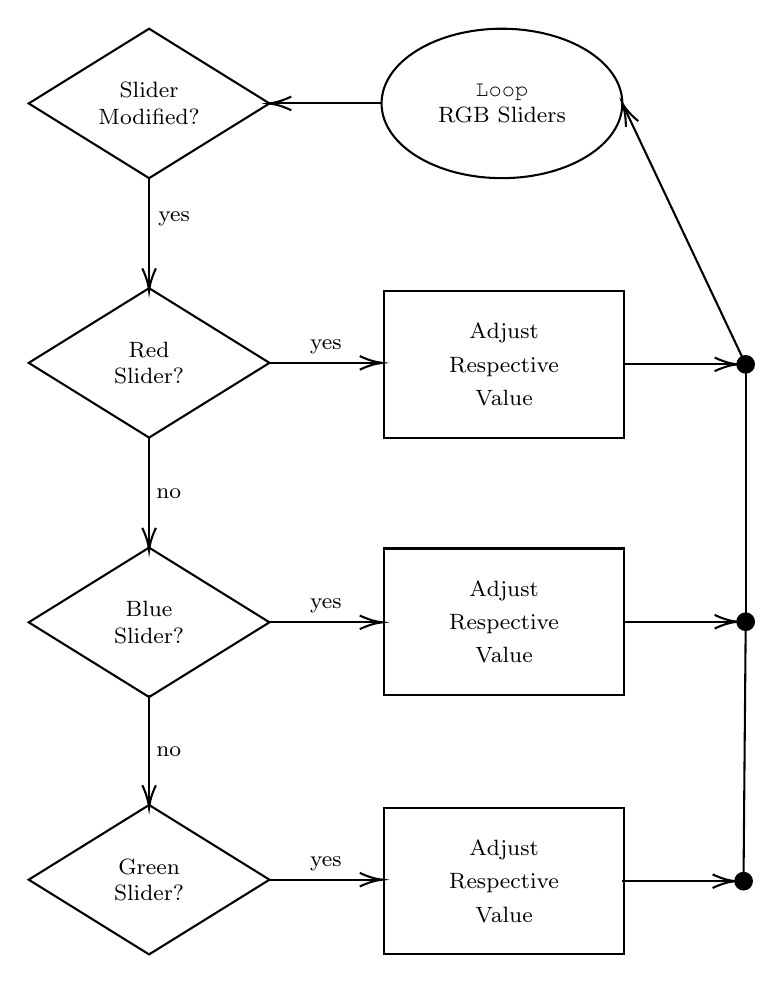
\begin{tikzpicture}[x=0.75pt,y=0.75pt,yscale=-1,xscale=1]
%uncomment if require: \path (0,499); %set diagram left start at 0, and has height of 499

%Shape: Ellipse [id:dp8829170838681932] 
\draw   (271,38) .. controls (271,18.12) and (296.97,2) .. (329,2) .. controls (361.03,2) and (387,18.12) .. (387,38) .. controls (387,57.88) and (361.03,74) .. (329,74) .. controls (296.97,74) and (271,57.88) .. (271,38) -- cycle ;
%Straight Lines [id:da5529521578911254] 
\draw    (271,38) -- (218.58,38) ;
\draw [shift={(216.58,38)}, rotate = 360] [color={rgb, 255:red, 0; green, 0; blue, 0 }  ][line width=0.75]    (10.93,-3.29) .. controls (6.95,-1.4) and (3.31,-0.3) .. (0,0) .. controls (3.31,0.3) and (6.95,1.4) .. (10.93,3.29)   ;
%Flowchart: Decision [id:dp3385459335713441] 
\draw   (159,2) -- (217,38) -- (159,74) -- (101,38) -- cycle ;
%Straight Lines [id:da5201076176684065] 
\draw    (159,74) -- (159,126.42) ;
\draw [shift={(159,128.42)}, rotate = 270] [color={rgb, 255:red, 0; green, 0; blue, 0 }  ][line width=0.75]    (10.93,-3.29) .. controls (6.95,-1.4) and (3.31,-0.3) .. (0,0) .. controls (3.31,0.3) and (6.95,1.4) .. (10.93,3.29)   ;
%Flowchart: Decision [id:dp392093801425095] 
\draw   (159,127) -- (217,163) -- (159,199) -- (101,163) -- cycle ;
%Straight Lines [id:da3794196322008889] 
\draw    (159,199) -- (159,251.42) ;
\draw [shift={(159,253.42)}, rotate = 270] [color={rgb, 255:red, 0; green, 0; blue, 0 }  ][line width=0.75]    (10.93,-3.29) .. controls (6.95,-1.4) and (3.31,-0.3) .. (0,0) .. controls (3.31,0.3) and (6.95,1.4) .. (10.93,3.29)   ;
%Flowchart: Decision [id:dp30939600166537806] 
\draw   (159,252) -- (217,288) -- (159,324) -- (101,288) -- cycle ;
%Straight Lines [id:da5744744656409009] 
\draw    (159,323) -- (159,375.42) ;
\draw [shift={(159,377.42)}, rotate = 270] [color={rgb, 255:red, 0; green, 0; blue, 0 }  ][line width=0.75]    (10.93,-3.29) .. controls (6.95,-1.4) and (3.31,-0.3) .. (0,0) .. controls (3.31,0.3) and (6.95,1.4) .. (10.93,3.29)   ;
%Flowchart: Decision [id:dp634645846033074] 
\draw   (159,376) -- (217,412) -- (159,448) -- (101,412) -- cycle ;
%Straight Lines [id:da38318286055379347] 
\draw    (217,163) -- (269.42,163) ;
\draw [shift={(271.42,163)}, rotate = 180] [color={rgb, 255:red, 0; green, 0; blue, 0 }  ][line width=0.75]    (10.93,-3.29) .. controls (6.95,-1.4) and (3.31,-0.3) .. (0,0) .. controls (3.31,0.3) and (6.95,1.4) .. (10.93,3.29)   ;
%Straight Lines [id:da8683490807016885] 
\draw    (217,288) -- (269.42,288) ;
\draw [shift={(271.42,288)}, rotate = 180] [color={rgb, 255:red, 0; green, 0; blue, 0 }  ][line width=0.75]    (10.93,-3.29) .. controls (6.95,-1.4) and (3.31,-0.3) .. (0,0) .. controls (3.31,0.3) and (6.95,1.4) .. (10.93,3.29)   ;
%Straight Lines [id:da45104646455767505] 
\draw    (217,412) -- (269.42,412) ;
\draw [shift={(271.42,412)}, rotate = 180] [color={rgb, 255:red, 0; green, 0; blue, 0 }  ][line width=0.75]    (10.93,-3.29) .. controls (6.95,-1.4) and (3.31,-0.3) .. (0,0) .. controls (3.31,0.3) and (6.95,1.4) .. (10.93,3.29)   ;
%Shape: Rectangle [id:dp09938506221224541] 
\draw   (272,128.42) -- (388,128.42) -- (388,199) -- (272,199) -- cycle ;
%Shape: Rectangle [id:dp9559172889746312] 
\draw   (272,252.42) -- (388,252.42) -- (388,323) -- (272,323) -- cycle ;
%Shape: Rectangle [id:dp7381524496015277] 
\draw   (272,377.42) -- (388,377.42) -- (388,448) -- (272,448) -- cycle ;
%Straight Lines [id:da3533613170972085] 
\draw    (387,412.71) -- (439.42,412.71) ;
\draw [shift={(441.42,412.71)}, rotate = 180] [color={rgb, 255:red, 0; green, 0; blue, 0 }  ][line width=0.75]    (10.93,-3.29) .. controls (6.95,-1.4) and (3.31,-0.3) .. (0,0) .. controls (3.31,0.3) and (6.95,1.4) .. (10.93,3.29)   ;
%Straight Lines [id:da6738025768509708] 
\draw    (388,287.71) -- (440.42,287.71) ;
\draw [shift={(442.42,287.71)}, rotate = 180] [color={rgb, 255:red, 0; green, 0; blue, 0 }  ][line width=0.75]    (10.93,-3.29) .. controls (6.95,-1.4) and (3.31,-0.3) .. (0,0) .. controls (3.31,0.3) and (6.95,1.4) .. (10.93,3.29)   ;
%Straight Lines [id:da6347872560204102] 
\draw    (388,163.71) -- (440.42,163.71) ;
\draw [shift={(442.42,163.71)}, rotate = 180] [color={rgb, 255:red, 0; green, 0; blue, 0 }  ][line width=0.75]    (10.93,-3.29) .. controls (6.95,-1.4) and (3.31,-0.3) .. (0,0) .. controls (3.31,0.3) and (6.95,1.4) .. (10.93,3.29)   ;
%Shape: Circle [id:dp403148021312002] 
\draw  [fill={rgb, 255:red, 0; green, 0; blue, 0 }  ,fill opacity=1 ] (442.42,163.71) .. controls (442.42,161.5) and (444.21,159.71) .. (446.42,159.71) .. controls (448.63,159.71) and (450.42,161.5) .. (450.42,163.71) .. controls (450.42,165.92) and (448.63,167.71) .. (446.42,167.71) .. controls (444.21,167.71) and (442.42,165.92) .. (442.42,163.71) -- cycle ;
%Shape: Circle [id:dp42109198635474243] 
\draw  [fill={rgb, 255:red, 0; green, 0; blue, 0 }  ,fill opacity=1 ] (442.42,287.71) .. controls (442.42,285.5) and (444.21,283.71) .. (446.42,283.71) .. controls (448.63,283.71) and (450.42,285.5) .. (450.42,287.71) .. controls (450.42,289.92) and (448.63,291.71) .. (446.42,291.71) .. controls (444.21,291.71) and (442.42,289.92) .. (442.42,287.71) -- cycle ;
%Shape: Circle [id:dp07663965283226659] 
\draw  [fill={rgb, 255:red, 0; green, 0; blue, 0 }  ,fill opacity=1 ] (441.42,412.71) .. controls (441.42,410.5) and (443.21,408.71) .. (445.42,408.71) .. controls (447.63,408.71) and (449.42,410.5) .. (449.42,412.71) .. controls (449.42,414.92) and (447.63,416.71) .. (445.42,416.71) .. controls (443.21,416.71) and (441.42,414.92) .. (441.42,412.71) -- cycle ;
%Straight Lines [id:da43770708123295354] 
\draw    (446.42,291.71) -- (445.42,408.71) ;
%Straight Lines [id:da595585539964409] 
\draw    (446.42,167.71) -- (446.42,283.71) ;
%Straight Lines [id:da6062871372734029] 
\draw    (446.42,163.71) -- (387.85,39.81) ;
\draw [shift={(387,38)}, rotate = 64.7] [color={rgb, 255:red, 0; green, 0; blue, 0 }  ][line width=0.75]    (10.93,-3.29) .. controls (6.95,-1.4) and (3.31,-0.3) .. (0,0) .. controls (3.31,0.3) and (6.95,1.4) .. (10.93,3.29)   ;

% Text Node
\draw (329,38) node  [font=\footnotesize] [align=left] {\begin{minipage}[lt]{47.62pt}\setlength\topsep{0pt}
\begin{center}
{\fontfamily{pcr}\selectfont Loop}\\RGB Sliders
\end{center}

\end{minipage}};
% Text Node
\draw (159,38) node  [font=\footnotesize] [align=left] {\begin{minipage}[lt]{38.1pt}\setlength\topsep{0pt}
\begin{center}
Slider\\Modified?
\end{center}

\end{minipage}};
% Text Node
\draw (162,93.5) node [anchor=west] [inner sep=0.75pt]  [font=\footnotesize] [align=left] {yes};
% Text Node
\draw (159,163) node  [font=\footnotesize] [align=left] {\begin{minipage}[lt]{28.12pt}\setlength\topsep{0pt}
\begin{center}
Red\\Slider?
\end{center}

\end{minipage}};
% Text Node
\draw (159,288) node  [font=\footnotesize] [align=left] {\begin{minipage}[lt]{28.12pt}\setlength\topsep{0pt}
\begin{center}
Blue\\Slider?
\end{center}

\end{minipage}};
% Text Node
\draw (159,412) node  [font=\footnotesize] [align=left] {\begin{minipage}[lt]{28.12pt}\setlength\topsep{0pt}
\begin{center}
Green\\Slider?
\end{center}

\end{minipage}};
% Text Node
\draw (161,226.21) node [anchor=west] [inner sep=0.75pt]  [font=\footnotesize] [align=left] {no};
% Text Node
\draw (161,350.21) node [anchor=west] [inner sep=0.75pt]  [font=\footnotesize] [align=left] {no};
% Text Node
\draw (244.21,160) node [anchor=south] [inner sep=0.75pt]  [font=\footnotesize] [align=left] {yes};
% Text Node
\draw (244.21,285) node [anchor=south] [inner sep=0.75pt]  [font=\footnotesize] [align=left] {yes};
% Text Node
\draw (244.21,409) node [anchor=south] [inner sep=0.75pt]  [font=\footnotesize] [align=left] {yes};
% Text Node
\draw (330,163.71) node   [align=left] {\begin{minipage}[lt]{43.1pt}\setlength\topsep{0pt}
\begin{center}
{\footnotesize Adjust}\\{\footnotesize Respective}\\{\footnotesize Value}
\end{center}

\end{minipage}};
% Text Node
\draw (330,287.71) node   [align=left] {\begin{minipage}[lt]{43.1pt}\setlength\topsep{0pt}
\begin{center}
{\footnotesize Adjust}\\{\footnotesize Respective}\\{\footnotesize Value}
\end{center}

\end{minipage}};
% Text Node
\draw (330,412.71) node   [align=left] {\begin{minipage}[lt]{43.1pt}\setlength\topsep{0pt}
\begin{center}
{\footnotesize Adjust}\\{\footnotesize Respective}\\{\footnotesize Value}
\end{center}

\end{minipage}};


\end{tikzpicture}
